\begin{song}{title=\centering Franky Dlouhán \\\normalsize Brontosauři  \vspace*{-0.3cm}}  %% sem se napíše jméno songu a autor
\moveright \stred \vbox{      %Varianta č. 1  ---> Jeden sloupec zarovnaný na střed	

\sloka 
	^{C}Kolik je smutného,
	
	když ^{F} mraky černé ^{C}jdou

	lidem nad ^{G}hlavou ^{F}smutnou dálavo^{C}u.
	
	Já slyšel příběh, který velkou pravdu měl,
	
	za čas odletěl, každý zapomněl.

\refren
	^{C}Měl kapsu ^{G}prázdnou Franky Dlouhán,

	po státech ^{F}toulal se jen ^{C}sám, a že

	byl ^{F}veselej, tak ^{C}každej měl ho ^{G7}rád.

	Tam ruce k ^{F}dílu mlčky přiloží a ^{C}zase

	jede ^{Ami}dál. A ^{F}každej kdo s ním

	^{G}chvilku byl, tak ^{F}dlouho ^{G7}se pak ^{C}smál.
	
\sloka	
	Tam, kde byl pláč, tam Franky hezkou píseň měl,
	
	slzy neměl rád, chtěl se jenom smát.
	
	A když pak večer ranče tiše usínaj,
	
	Frankův zpěv jde dál nocí s písní dál.\elipsa\dots
	
\sloka
	Tak Frankyho vám jednou našli, přestal žít,
	
	jeho srdce spí, tiše smutně spí.
	
	Bůh ví jak, za co tenhle smíšek konec měl,
	
	farář píseň pěl, umíraček zněl.\elipsa\dots

}
\setcounter{Slokočet}{0}
\end{song}


\begin{figure}[h]
\centering
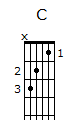
\includegraphics[scale=1.5]{../Akordy/c.png}
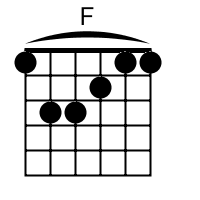
\includegraphics[scale=1.5]{../Akordy/f.png}
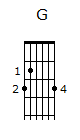
\includegraphics[scale=1.5]{../Akordy/g.png}
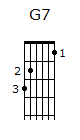
\includegraphics[scale=1.5]{../Akordy/g7.png}
\end{figure}
	